\chapter{Load- and Locality-Aware Load Balancing}
\label{chap:chrlu}

% While serverless computing provides more convenient abstractions for developing and deploying applications, the Function-as-a-Service (FaaS) programming model presents new resource management challenges for the FaaS provider. 
In this chapter, we investigate load-balancing policies for serverless clusters and find that the locality vs. load tradeoff is crucial and presents a large design space.
Locality, i.e., running repeated invocations of a function on the same server, is a key determinant of performance because it increases warm-starts and reduces cold start overheads.
Many functions are too popular and running all their invocations on one worker will overload it, requiring us to sacrifice locality and spread their invocations across the cluster.
We find that the locality vs. load tradeoff is crucial and presents a large design space. 

We enhance consistent hashing and bring it to FaaS, developing CH-RLU: Consistent Hashing with Random Load Updates, a simple, practical load-balancing policy which provides more than $2\times$ reduction in function latency. 
Our policy deals with highly heterogeneous, skewed, and bursty function workloads, and is a drop-in replacement for OpenWhisk's existing load-balancer.
We leverage techniques from caching such as SHARDS for popularity detection, and develop a new approach that places functions based on a tradeoff between function locality, cluster load, and randomness. 


\section{Background: Load Balancing}

Managing the load of a cluster of servers is a common problem in distributed computing systems.
Load-balancing policies typically rely on some notion of ``load'' of a server, such as the number of concurrently executing tasks, length of the task-queue, cpu-utilization, etc.
%
The first broad class is \emph{compute-oriented} load-balancers, typically used for short-running tasks and queries. 
Load-balancing for computational tasks is common in scenarios like web-clusters~\cite{karger1999web}. 
In these systems, the tasks can be executed on any server,  servers in a cluster are largely fungible, and the task performance largely depends on the server-specific cpu-utilization at the time.

Load-balancing techniques have received significant theoretical attention (especially using queuing theory), as well as many practical systems~\cite{decandia2007dynamo}. 
From a queuing theory perspective, policies such as least-work-left (LWL) and Join-Shortest-Queue (JSQ), have studied near-optimal load balancing for computing load-dependent workloads under a processor-sharing (PS) setting. 

Interestingly, load-balancing for \emph{data-oriented} systems, such as Content Delivery Networks (CDNs)~\cite{nygren2010akamai}, and distributed key-value stores (such as Amazon Dynamo~\cite{decandia2007dynamo}) must also balance the load on servers, but with data locality as a key requirement.
In this context, locality refers to requests for the same object being handled by the server, or the same subset of servers if the object is replicated. 
We find that FaaS load balancing requires and benefits from \emph{both} these objectives: minimizing computing load \emph{and} maximizing locality to reduce cold starts. 

\begin{comment}
However, combining compute-oriented load-balancing solutions 

In large clusters, consistent load information cannot always be assumed, and simple techniques work well in practice.
For instance, the power of two random choices, which schedules a task on the least loaded of two random servers. 

Queuing analysis?
- G/G/PS system. Greedy load balancing is sub-optimal.

Randomization and power of 2 choices is popular.

But arent locality aware.

Web server load balancing work. A Gandhi etc. 
\end{comment}

%\vspace*{-0.2cm}
\subsection{Consistent Hashing} 
\label{subsec:ch}

\begin{figure}
  \centering
  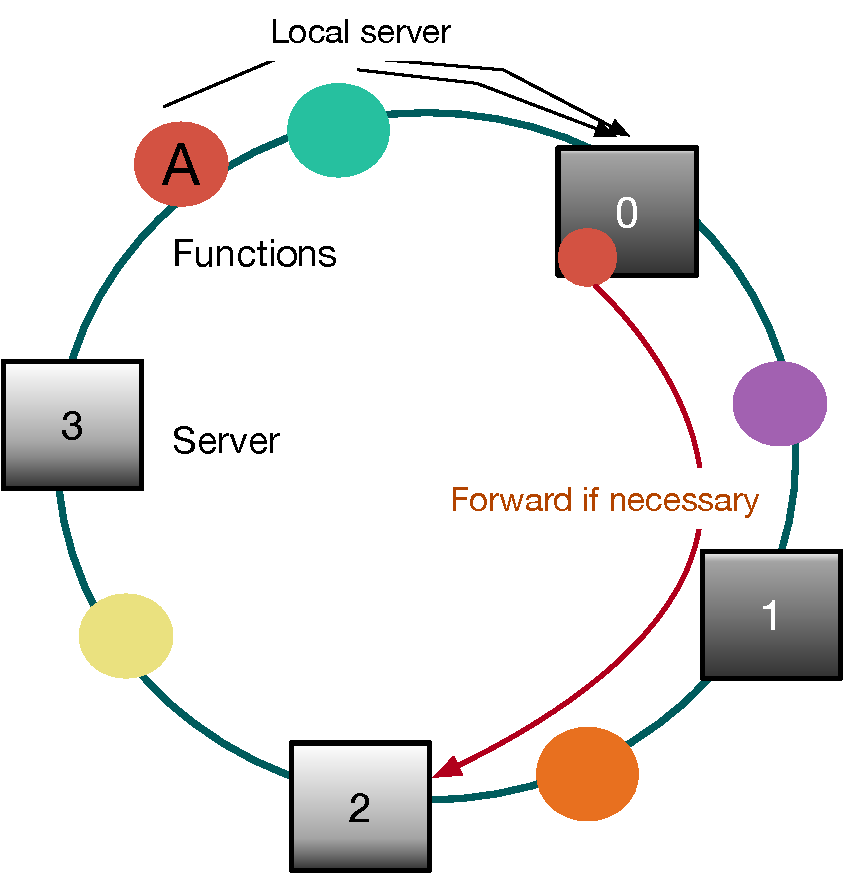
\includegraphics[width=0.7\textwidth]{chrlu/faaslb-osdi22/figs/ch-bl.pdf}
%  \vspace*{-0.2cm}
  \caption{Consistent hashing runs functions on the nearest clockwise server. Functions are forwarded along the ring if the server is overloaded.}
  \label{fig:ch}
%    \vspace*{-0.2cm}
\end{figure}

For data-oriented systems, a common technique to ensure locality is Consistent Hashing~\cite{karger1999web, karger1997consistent}.
Objects are mapped to servers based on some object id or key.
Consistent hashing preserves object-server mapping even in the face of server additions and removals, which improves locality.
%
Figure~\ref{fig:ch} provides an overview of consistent hashing. Both objects and servers are hashed to points on a ``ring'', and objects are assigned to the next server (in the clockwise direction) in the ring. 
Addition or removal of servers only affects the nearby objects by remapping them to the new next server in the ring.

OpenWhisk uses a modified consistent hashing algorithm for its default load balancer.
As functions are sent to servers, their expected memory footprint is added to a server-specific running counter of outstanding requests.
Upon completion the memory size of a function is decremented from that server's counter.
If the counter for a function's \quotes{home} server would exceed the assigned memory on the server it is forwarded along the ring.
%
The drawback of this policy, and consistent hashing as a whole, is that the performance can be affected by the relative popularities of the different objects.
A highly popular object can result in its associated server getting overloaded.
This problem is exacerbated in the case of FaaS functions, as we shall demonstrate in the next section. 


\section{Load-aware Consistent-Hashing} % Based Load Balancing Policies}
\label{sec:chrlu}

In this section, we describe the load-balancing algorithm which is locality, stale-load, and burst aware.
We assume a cluster  homogeneous servers, and 
a new function invocation can be sent to any of the servers.
Each server implements keep-alive for functions: after successful execution, the function's container is stored in server memory, and evicted based on some eviction policy. % such as LRU, TTL, or Greedy-Dual~\cite{faascache-asplos21}. 
%Subsequent invocations of the function constitute  a ``warm'' start which is significantly faster than a cold start. 
%The keep-alive policy determines when and which functions to evict when the server memory is fully occupied by running and ``warm'' containers.

% Thus, locality is crucial for achieving low latency.
% Data storage clusters such as distributed key-value stores also require object-access requests to be routed to the same set of servers.
% However, locality is a stronger constraint in data storage because of consistency requirements. 
% In the case of functions, locality is preferable, and server loads are also considered. 

% Where is the queuing theory perspective? LWL/ SJF/ dispatch. Highly variable job lengths.
%\vspace*{-0.2cm}
\subsection{Tradeoff between Locality and Load}

We use consistent hashing as the fundamental principle to ensure high locality: repeated invocations of the same function occur on the same server. 
However, popular functions, i.e., which are invoked very frequently, can result in overloaded servers.
Because function performance is affected by server load and resource availability, focusing on locality alone can result in slow function execution.

Function popularities are also highly skewed: a small percentage account for a vast majority of invocations.
With pure locality-based load-balancing, the servers of these popular functions would be severely overloaded.
Functions also can run for significantly longer than simple web requests, and thus they impose more load on servers, and the cost of a wrong placement decision is higher. 
This, combined with bursty invocations, can significantly increase the tail latency of functions. 
Thus pure-locality policies such as classical consistent hashing are not sufficient, and 
our research question is: \emph{Can consistent hashing be used to reduce latency due to overloaded servers?} 
Or put another way, can we balance the tradeoff between function locality and server-loads with consistent hashing? 


Our key idea is to extend consistent hashing to take also into account server loads, the cold start overheads of different functions, and the bursty traffic that is a key characteristic of FaaS workloads.
In the rest of this section, we describe our approach. 

% \subsection{Broad design Criteria}
% LB latency is important: millisecond pricing, so LB cant take up too many cycles.

%\vspace*{-0.2cm}
\subsection{Key Principle: Load-based Forwarding}

To balance the locality vs. server load tradeoff, we build on a new variant of consistent hashing called Consistent Hashing with Bounded Loads~\cite{mirrokni2018consistent} (abbreviated as CH-BL in the rest of the chapter).  
The key idea behind CH-BL is to use consistent hashing to locate servers for objects, and if the servers are ``full'', then ``forward'' the objects to the next server in the consistent hashing ring.

For example, in Figure~\ref{fig:ch}, function A is originally assigned to server 0, but this ``home'' server is overloaded (already running many functions), and thus the function is forwarded along the ring until a suitable non-overloaded server (2) is found. 
Any 5-independent hashing function can be used for determining the ``home'' server of a function. %which is determined by hashing the function's unique id. 
Users can specify the load upperbound or the capacity of the server ($b$), which determines the max load the server can sustain.  
Consistent hashing with bounded loads provides many strong theoretical guarantees on the length of the forwarding chain until the object is safely placed on a server. 


Interestingly, forwarding along the ring not only avoids server overloads, but also improves locality, \emph{even in overload scenarios.}
Forwarding along the ring has the advantage that even if function is not run on its ``home'' server, subsequent invocations that ``overflow'' still have a high warm-start probability on the servers on the overflow chain. %, with the warm-start probability decreasing in chain-length.
The warm-start probability is highest on the home server, and decays the farther the function is from its home server. 
This is more beneficial than alternative techniques such as Consistent Hashing with Random Jumps~\cite{chrj-aaai21}, which do not preserve locality and instead forwards to randomly chosen least loaded servers. 

%\vspace*{-0.2cm}
\subsection{Server Load Information}

Server load is a key metric in load-balancing policies.
We need to be able to determine the \emph{relative} suitability of one server over another, and thus many existing metrics can be used to provide information about server loads.
%
Simple metrics such as number of running functions are insufficient, since functions can have highly variable execution times. 
OpenWhisk currently uses occupied-memory used by active/running invocations as a proxy for load, and is unsuitable for the same reason. 
Both these metrics fail to capture CPU loads and lead to scalability issues when used by the load-balancer. 


% OpenWhisk currently uses occupied-memory as a proxy for load.
% However both these approaches require the load-balancer to keep accurately track of which function invocations and \emph{completions} on each server, which creates a scalability bottleneck.
% Furthermore, using memory availability is not suitable for resource-conserving keep-alive policies such as LRU or Greedy-Dual, which have been shown to be much more effective than OpenWhisk's default Time-to-Live (TTL) based eviction.


Instead, we primarily rely on \emph{system-level} load metrics, such as the standard Linux 1-minute load-average.
In addition to CPU utilization, this also captures the I/O wait due to cold starts, and provides a more realistic measure of load.
Traditional Linux load-average estimates the total number of processes running and ready-to-run, and we normalize the load-average by the number of CPUs. 
Thus, a load-average of $8$ on an 8 core server (discounting hyperthreading) is normalized to 1. 

An important practical consideration is that load information is often \emph{stale}, with the degree of staleness ranging from a few seconds to several minutes. 
For instance, because the Linux load average is an exponential moving average, it is slow to change.
Furthermore, load monitoring and reporting has delays due to how frequently the metrics are gathered at the local server, and how often they are made available to the load-balancer.
We use a simple publish-subscribe-like system, where individual servers periodically (every 5 seconds) push their load information, and the load-balancer uses these published loads to make all scheduling decisions.


%\subsection{Cold start Aware Bounded-Loads

%\vspace*{-0.2cm} % Challenges of CH-BL adoption. 
\subsection{Why CH-BL Is Insufficient}

The high computing load of functions, their bursty nature, and the staleness of loads, are the three major challenges to Consistent Hashing with Bounded Loads~\cite{mirrokni2018consistent} that the original algorithm is not designed to meet. 
There are a few practical considerations and key differences between simple object/storage caching and function execution:
1. CH-BL does not take into account the heterogeneity in running times and memory size of the objects (i.e., functions).
2. The implicit CH-BL performance model is binary: running-time is assumed to be uniform as long as servers are under the load-bound. 
3. The server loads evolve as a result of the actual function execution and are not just uniformly incremented as in the original algorithm. Object deletions are also not handled explicitly: we let the lazily computed load average determine whether a server meets the load-bound or not. 

\emph{Importantly, we do not assume complete and consistent state information about the servers.}
Omniscient knowledge of the execution state of all functions running all servers can certainly be leveraged effectively to run functions on the most suitable server.
However, such maintaining such global knowledge is expensive and impractical as far as storage consistency and latency are concerned.
Thus, we are striving for load-balancing policies which are robust to stale, incomplete, and coarse-grained information about server states. 
In the rest of this section, we shall show how the above three limitations of CH-BL can be overcome in FaaS load-balancing settings. 

%\vspace*{-0.4cm}
\subsection{Incorporating Function Performance Characteristics}
\label{subsec:chch}


Different running time and performance characteristics of functions can be incorporated into consistent hashing.
\emph{The key problem is to determine when and which function to forward.}
The forwarding policies need to be cognizant of the warm and cold running times, and the sensitivity to load of different functions. 

%Each server has a load-bound which we do not want the server's load to exceed. As described in the previously, consistent hashing with bounded loads can ensure that no individual server exceeds the load-bound $c$, by forwarding the request (in our case, function invocation) to the next server in the ring, until a suitable server is found. This bound determines what the maximum load of the servers will be. 


Assume a load-bound of $b$, the warm time of a function is $w$, and the cold time is $c$ (slow-start). 
%
The current or the home server will be ``0'', and the next server in the ring that the function may be forwarded-to will be denoted by ``1''. 
Running it on the ``home''/local server will result in expected time $E[T_0] = (p_0w+(1-p_0c)S(L_0) $, where $p_0$ is the cache-hit/keep-alive probability, and $S(L_0)$ is the slowdown in function if the load on the server is $L_0$. 
When a function in invoked the load balancer has the choice to either run in on the home server or forward it to the next server, where it is less likely to be found in the keep-alive cache, because the reuse-distance is much larger for the servers down the chain.
Therefore we can compute the forwarding regret, $E[T_0]/E[T_1]$.

The properties of bounded-loads allows us to easily compute this value.
The probability of being forwarded is small, and is $1/b$ based on Lemma 4 of~\cite{mirrokni2018consistent}.
The reuse-distance of the function, and hence the hit-rate on the original/home server will be larger: $p_0 > p_1*b$. 
% Based on our empirical observation of sub-linear performance decrease due to load (Section~\ref{subsec:function-perf}), in the worst case, the home server will be overloaded and alternative server will not be, and hence the ratio of slowdowns, $S(L_0)/S(L_1) > b$.
Based on our empirical observation of sub-linear performance decrease due to load (elided for space), in the worst case, the home server will be overloaded and alternative server will not be, and hence the ratio of slowdowns, $S(L_0)/S(L_1) > b$.
%
Minimizing the regret, we get that the function should be forwarded if $L>cb/w$.
Thus, the effective load upper-bound is \emph{increased} by a factor of $\text{cold}/\text{warm}$  time, allowing us to run more functions per server. 
In our empirical evaluation, we will show that this can significantly improve performance over plain CH-BL with a function-agnostic constant load-bound.
If the cold and warm times of a function are not available, then they are assumed to be equal, thus this degrades to classic function-agnostic bounded-loads. 


%%%%%%%%%%%%%%%%%%%%%%%%%%%%%%%%%%%%%%%%%%%%%%%%%%%%%%%%%%%%

%\vspace*{-0.4cm}
\subsection{Handling Bursts}
\label{subsec:bursty}

Functions come in a variety of frequency classes and are also prone to unpredictable burstiness (i.e., very low inter-arrival-times for a short duration). 
Identifying these bursts and both keeping latency for such \quotes{popular} functions low and preventing them from negatively impacting co-located functions is critical.
We have found that handling overload conditions is a key requirement and can significantly affect the tail latency.

Bursty function invocations result in two main problems.
First, they cause an increase in server load beyond the actual load-bound, because load is only lazily tracked.
The delayed load information can result in a popular function completely overwhelming a server, causing load \quotes{hotspots} in the cluster.
The second problem is that in extreme cases, the inter-arrival-time is less than the function latency, causing concurrent invocations.
Even if these concurrent invocations are run on a \quotes{local} server with the function present in the keep-alive cache, there will still be cold starts, since each invocation must run in its own container. 

Our solution to these two problems caused by bursty invocations is to detect popular function bursts, ``spread'' these invocations around multiple servers to prevent cluster hot-spots, and use stochastic/random load updates to introduce randomness into the load-balancing. 

\begin{comment}
Multiple problems. 1. Increase the load beyond the bound because lazily tracked. 2. Concurrent: no warm starts. Spreading them around will be useful. 

The problem of concurrent invocations is vexing even with locality, since containers may be in use and thus results in cold starts for these invocations. In the worst case we must accept $n-1$ cold starts for an $n$ core server. 

% Very popular functions can present problems.
We use two strategies:
1. Identify popular functions in a low-overhead online manner.
1a. Use this information to inform the load estimate. Due to the problem of \textbf{stale loads.}
2. Extreme overload: pick least loaded server if going around the horn.  % this seems orthogonal. 

This is similar to epsilon-greedy: we greedily pick the server based on the expected running time estimate for unpopular functions and probabilistically for popular functions. 
The probability is determined based on the server load and the noise in the server load estimate, which in turn depends on the estimate of the recent arrival rate of the functions. 

\end{comment}

%\vspace*{-0.2cm}
\subsubsection{Detecting Popular Functions with Spatial Sampling}

Our goal is to detect ``popular'' functions with low inter-arrival-times, in an online low-overhead manner.
%
Popularity detection must take into account the changing invocation frequencies of different functions over time, and be low-overhead.
We identify the top \textit{p} percentile of functions by their inter-arrival-times (IAT), or below some explicit IAT threshold, to reduce unnecessary hyperparamaters. 

Our approach is general: we first build a histogram of inter-arrival-times using sampling, and then query it. 
We note similarities with computing reuse-distance histograms, which are the building block of miss-ratio curves. 
%Our goal is to find the popular functions that have a low inter-arrival-time (IAT) quickly.
Reuse-time histograms are a simpler version of reuse-distances.
Recall that reuse distance is the number of \emph{unique} objects accessed, whereas inter-arrival-time is simply the difference in wall-clock times.
%In particular, we use the SHARDS technique, and modify and simplify it to compute an approximate IAT distribution instead of a reuse distance distribution. 



Our solution to identifying popular functions and function bursts is inspired by the popular SHARDS~\cite{shards} algorithm for building reuse-distance histograms. 
%
Following SHARDS, we randomly sample invocations to track individual function IATs. 
This tracking is simplified by only recording the most recent access time, and then computing the IAT as an estimated moving average of the current IAT and  $now - last\_access$. 
These values are tracked for every function, and functions in the top $p^{th}$ percentile of IATs are considered \textbf{popular}.
%
For the sampled functions using spatial hashing, we update their IAT.
Note that this approach keeps only a small number of last-accessed-iat entries in memory: ``have-been'' popular functions are naturally evicted from the tracking list. 
Because we do not care about reuse-distances, we avoid keeping a tree of reuse-distances, resulting in a simplified SHARDS-like algorithm (see Algorithm~\ref{algo:shards-popular}). 


% \begin{lstlisting}
% def update_shards_popular(func, time):

% if Ti < T:
%   if func in last_access_times:
%     # Already in our sample set 
%     iat = (t-last_access_times[func])/R 
%     last_access_times[func] = t 
%     prev_iat = iat_dict[func]
%     iat_dict[func] = iat 
%     iat_heap.remove((prev_iat, func))
%     iat_heap.push((iat, func))
%   else:
%     #First access... iat=='inf'
%     last_access_times[func] = t 
%     iat_dict[func] = t/R 
%     iat_heap.push((t/R, func))
%   iats_only = [x[0] for x in h]
%   pop_thresh = percentile(iats_only, 20)
%   avg_iat = percentile(iats_only, 50)
%   avg_arrival_rate = 1.0/(1000.0*avg_iat)
% \end{lstlisting}

\begin{algorithm}
% \begin{algorithmic}
\caption{SHARDS-inspired popular function detection. Functions with the top p percentile of IATs are 'popular'.}
\begin{algorithmic}[1]

  \Procedure{update\_shards\_popular}{$func, time$}
 \State $P \gets 100.0$
 \State $T \gets 20.0$ 
 \Comment{Effective sampling rate}
 \State $R \gets T / P$ 
 \State $Ti \gets abs(hash(func.name))$ 
 \If{$Ti \leq T$}
  \If{$last\_access\_times.contains(func)$}
  \Comment{Already in our sample set} 
  \State $iat \gets (t-last\_access\_times[func])/R$
  \State $last\_access\_times[func] = t$ 
%  \State $prev\_iat = iat\_dict[func]$
%  \State $iat\_dict[func] = iat$
%  \State $iat\_heap.remove((prev\_iat, func))$
  \State $iat\_heap.push((iat, func))$
  \Else
  \Comment{First access... iat=='inf'}
  \State $last\_access\_times[func] = t$
%  \State $iat\_dict[func] = t/R$
  \State $iat\_heap.push((t/R, func))$
  \EndIf
 \EndIf
 \State $iats\_only \gets iat\_heap.values()$
 \State $pop\_thresh \gets percentile(iats\_only, p)$
% \State $avg\_iat \gets percentile(iats\_only, 50)$
%  \State $avg\_arrival\_rate \gets 1.0/(1000.0*avg\_iat)$
\EndProcedure
\end{algorithmic}
\label{algo:shards-popular}
\end{algorithm}

%\vspace*{-0.2cm}
\subsubsection{Randomly Updating Stale Loads}

Popular functions represent such a large percentage of invocations yet a small number of functions, that they can be safely spread across many servers without causing cold starts.
A fair load balancing algorithm must spread popular functions to ensure QoS for less frequent functions. 
Because load information is stale, adhering to locality and load can result in servers facing a herd-effect.
Randomization is a powerful strategy to ameliorate such effects, however, we must use it judiciously because of the strong effects of locality in FaaS load-balancing.

Our solution is to introduce random forwarding (along the ring) which is proportional to the load of the server, such that popular functions are forwarded with a higher probability. 
If the (stale) load of the server is $L$, we update its load by adding gaussian noise with a mean of the \emph{extra anticipated load} on the server based on the staleness and function arrival rate on the server ($\lambda$).
Specifically, the $L_{\text{noisy}}=L+\mathcal{N}(\mu=\lambda, \sigma=0.1)$, where $\mathcal{N}$ is a Gaussian random variable. 
For popular functions, we  compare the $L_{\text{noisy}}$ to the load-bound.
For remaining functions, we continue to use the stale load $L$. 
Thus for highly loaded servers ``near'' the upper-bound, the extra random noise will result in the popular bursty functions being forwarded more, to avoid the herd-effect.

\begin{comment}
To achieve this, we introduce Gaussian noise to the forwarding decision.
% is added to the load based on the iat and the rate. Per-function noise. Can also be just a per-server estimate if desired. 
We compute the global arrival rate, then estimate the per-server arrival rate and the effect an invocation has on server load, following the steps in Algorithm~\ref{algo:PopularRLUPolicy}.
For each server we then sample noise from the normal distribution whos mean is centered on the \textit{extra\_anticip\_load}, and add that to the server's tracked load to get \textit{Lnoise}.
We iterate along the ring of servers until we find one with a \textit{Lnoise} less than the global \textit{bounded\_ceil}.
In the case where we skip over 3 servers, we assume that the invocation will run cold no matter what, and assign it to the least loaded server.
\end{comment}

% \textbf{Question 1:} Why not do the stale load error correction for all functions, why just the popular ones?

% \begin{figure}
\begin{algorithm}
  \caption{Random Load Update Forwarding Function}
  \begin{algorithmic}[1]
    \Procedure{CH-RLU-forward}{$func, server, chain\_len $}
    \State $b, b\_max, max\_chain\_len \gets system\_params $
    \If{$ chain\_len > max\_chain\_len $}
    \State return least-loaded-server
    \EndIf 

    \State $\lambda \gets 1.0 / avg\_iat$ \Comment Computed from Algorithm~\ref{algo:shards-popular}
     \State $L=Load(server)$
    \If{popular(func)} \Comment Computed from Algorithm~\ref{algo:shards-popular}
         \State $L = Load(server) + \mathcal{N}(\mu=\lambda\,\sigma=0.1)$
    \EndIf 
    \If{$L < min(cb/w, b\_max)$}
       \State server
    \Else \State CH-RLU-forward(func, next(server), chain\_len+1)
    \EndIf
    \EndProcedure
    \end{algorithmic}
\label{algo:PopularRLUPolicy}
\end{algorithm}

%\vspace*{-0.2cm}
\subsection{Putting it all together: CH-RLU}
\label{subsec:chrlu:together}

Our overall policy, Consistent Hashing with Random Load Updates (CH-RLU), combines all the previously described techniques and insights. 
When a new invocation arrives, we query the popular IAT threshold to determine what class of function it is. 
Functions are distributed via Algorithm~\ref{algo:PopularRLUPolicy}, which combines the use of SHARDS for popularity detection, cold and warm times for increasing the effective load-bound, and noisy loads. 
We bound the cold/warm ratio with a final load upper-bound b\_max.
The load bound parameters determine the locality-sensitivity: higher values of b and b\_max increase locality at the risk of resource-contention delays.
Similarly, higher values of $p$ results in more aggressive random forwarding and reduces locality. 


Forwarding along the chain has diminishing returns of locality, and if the function gets forwarded more than max\_chain\_len times, we simply run it on the least-loaded server. 
%
If the least loaded server is also overloaded, we drop the function. 
We have also implemented a simple PID controller with hysteresis for horizontal scaling, by using server load averages as the input control signal. 
This horizontal scaling is conservative, with a large dead-band of 5 minutes, and scaling is triggered only if the at least 50\% of the servers are overloaded.
As we shall show in the empirical evaluation, CH-RLU significantly reduces the variance in the loads among servers, and thus is more amenable to this horizontal scaling policy. 

% Unpopular functions still use Algorithm~\ref{algo:ConsistentCachePolicy}.
% In all cases, if we exhaust the list of servers trying to find one with low load, we randomly assign the invocation to a server.
% This only occurs in the most extreme cases of system load and also prevents spamming a popular server in that same scenario.



% if popular: L+Noise > bound 
% else: L > bound 

%%% Local Variables:
%%% mode: latex
%%% TeX-master: "paper"
%%% End:


%\vspace*{-0.2cm}
\section{Implementation}
\label{sec:impl}

We have implemented our consistent hashing with random load update (RLU) policy and other load-balancing policies in OpenWhisk, a popular FaaS system.
Our changes amount to more than 1,700 lines of code across many OpenWhisk components, but are primarily in the load-balancer class. 
In this section, we describe major implementation details, as well as key performance optimizations which significantly improve OpenWhisk performance and scalability by more than $4\times$. 

Our policies are implemented by modifying the load-balancer module of OpenWhisk (see Figure~\ref{fig:sys-diag}).
CH-RLU is implemented by modifying the existing OpenWhisk ``container sharding'' policy, which also uses consistent hashing, and forwards functions using only available memory as the load metric.
We use OpenWhisk's existing consistent hashing implementation, permiting an ``apples to apples'' comparison, and also making CH-RLU a ``drop-in'' replacement for the OpenWhisk default load-balancing. 
At the invoker level, we adapt FaasCache's GreedyDual keep-alive policy, which increases the keep-alive effectiveness compared to OpenWhisk's default non-resource-conserving TTL eviction~\cite{faascache-asplos21}. 

\begin{figure}  
  \centering
  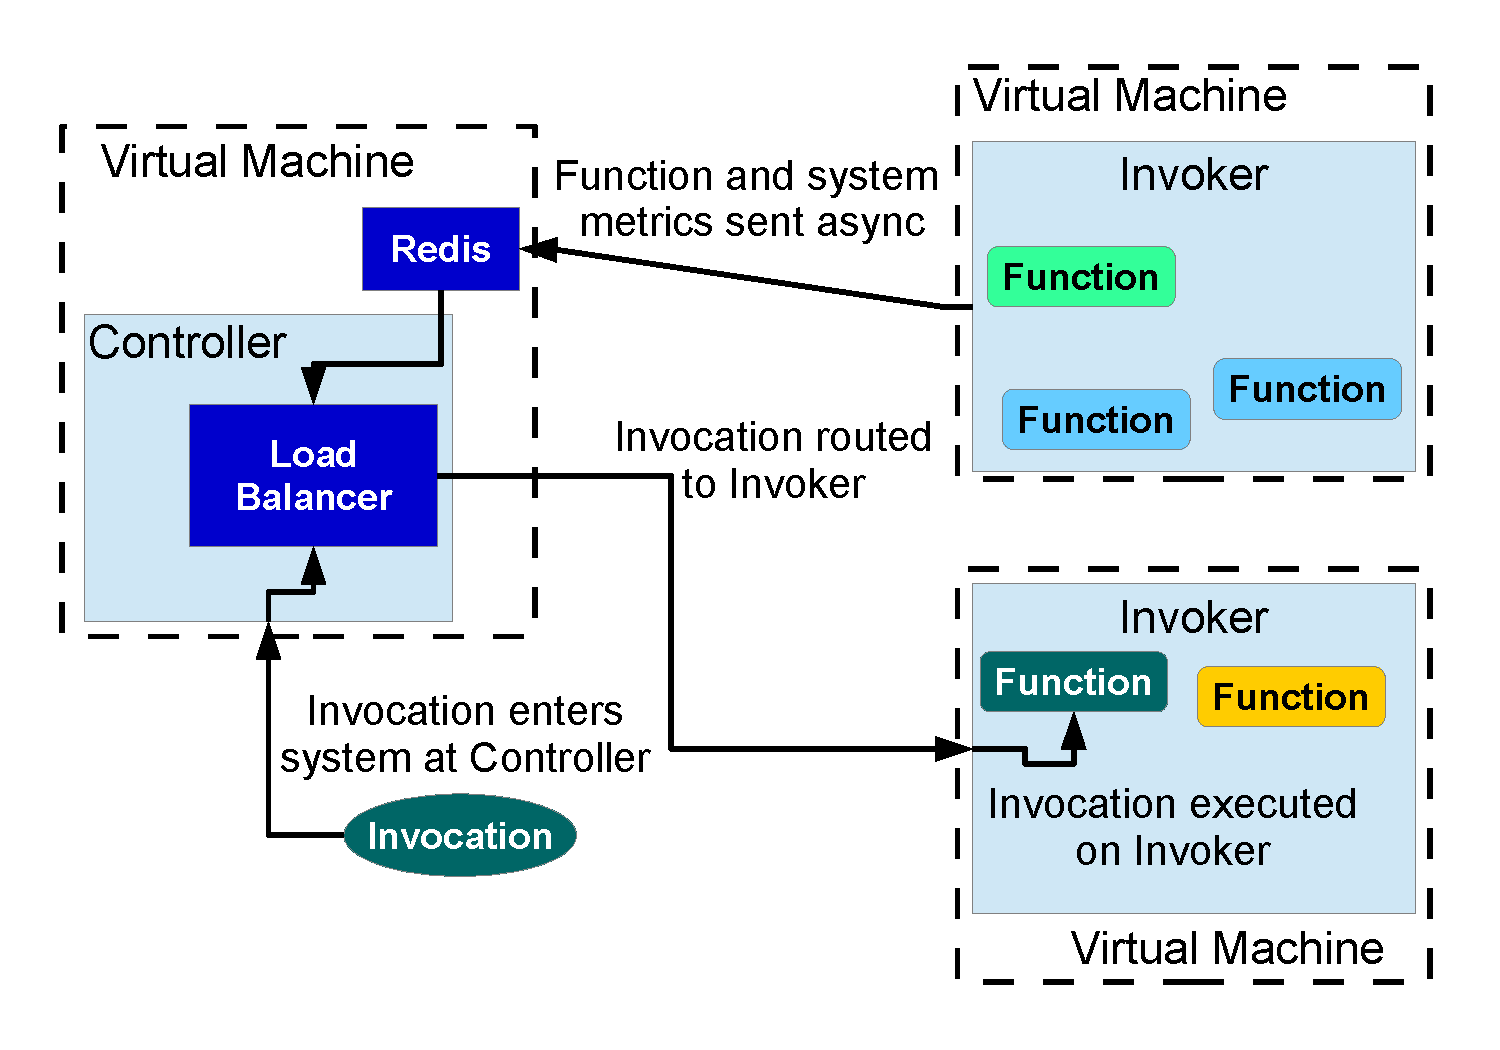
\includegraphics[width=0.6\textwidth]{chrlu/faaslb-osdi22/figs/sys-diag.pdf}
 %   \vspace*{-0.3cm}
  \caption{System diagram of relevant OpenWhisk components and communication used to schedule and run function invocations.}
  \label{fig:sys-diag}
  %  \vspace*{-0.3cm}
\end{figure}

The CH-RLU algorithm described in the previous section requires two main additional pieces of information from each invoker/server: the load averages, and the cold/warm running times of functions. 
Both of these are periodically (every 5 seconds) captured and stored in a centralized redis key-value store.
The load-balancer in the controller reads these asynchronously: working with stale and inconsistent metrics is our key design goal. 
The default load-bound, b, is 1.2, and the max load, b\_max is 6. Popularity threshold is set to 20\%.
We did not observe performance to be very sensitive to these parameters, and thus do not need to auto-tune them, and they are suitable as user-inputs. 

%\vspace*{-0.2cm}
\subsection{Performance Optimizations For OpenWhisk}

Since our goal is to run functions under high load, we ran into a large number of OpenWhisk performance and scalability bottlenecks.
We found default OpenWhisk to be almost unusably slow and unstable even under reasonable load. 
We present their details and our actions to overcome them, hoping that the fast-growing serverless computing research field can benefit from our lessons. 


In our experience, the primary source of scalability bottlenecks when concurrently managing Docker containers.
We found significant contention in \texttt{dockerd}, Docker's control daemon which handles all the container lifecycle events.
Even at moderate loads (normalized server load average close to 1), high dockerd contention can increase tail latencies by \emph{several minutes!}


Currently, OpenWhisk \textbf{pauses} each container after function execution, which prevents it from being scheduled by the CPU.
It then resumes the container before running the next invocation of the same function (assuming a warm start).
Each invocation therefore requires these two additional (pause/resume) events to be handled by dockerd, which results in significant lock contention.
Because of the FaaS programming model, the pausing is not necessary, since nothing in the container can run after a function has returned.
Therefore, we remove these redundant pause/resume operations to reduce dockerd contention.
This reduces the OpenWhisk overhead by 0.2 seconds \emph{per-invocation} on average.
More importantly, by reducing dockerd contention, we were able to run a much larger number of concurrent functions. 

An even larger source of scalability bottleneck is \textbf{network} namespace creation time.
Using the default bridge networking requires each invocation to create a new TUN/TAP network interface.
We found this to be a very expensive operation because of Linux network stack overheads (several 100 ms), and because of dockerd's userspace lock (futex) contention for its networking database. 
We found that as the \emph{historical} total number of containers launched grows, so does the size of the network-interface database.
Dockerd reads and updates this database under the critical section, and the larger database results in higher lock contention.
As a result, we were unable to use VMs/servers with more than 4 CPUs after 20 minutes of sustained load, since the dockerd contention resulted in many functions timing out (timeout was 5 minutes)! 

We sidestep this problem by not using bridge networking, but instead using Docker's \textit{host} network option and assigning each container a unique port on the host. 
Implementing the network change required updating the OpenWhisk runtimes used to wrap functions to monitor their specified port.
This change allowed us to run functions on larger invokers and under more sustained load, and eliminated most timeouts. 

Finally, after a certain request rate threshold, we found the default \texttt{nginx} OpenWhisk frontend would crash and return \textit{502 BAD GATEWAY} for all URLs. 
We did not discover the cause of this problem, and simply bypassed it by letting function invocations to communicate with the controller/load-balancer directly. 

\noindent \textbf{CPU limits.} 
OpenWhisk uses the \textit{-{}-cpu-shares} option to set container CPU priority.
This has an unintended consequence of allowing functions to use more than one CPU core while running.
Major FaaS providers constrain functions to a single core unless they have extremely high memory allocations (<1 GB).
In order to stay in line with providers and prevent outsized impact on system load from some functions, we use the \textit{-{}-cpus} flag instead to assign each function no more than one CPU.

Together, these performance optimizations have allowed us to run OpenWhisk on invokers that are $4\times$ larger, and serve more than $6\times$ the load, without dropping functions due to timeouts.
%
We plan to upstream all these performance optimizations in OpenWhisk to provide a higher-performance and lower-jitter control plane for FaaS research and production deployments. 

\begin{comment}
\noindent \textbf{docker pause.} 
OpenWhisk pauses Docker containers after each invocation completes to prevent the user code from continuing to run.
We disable this pausing because it causes significant contention inside Docker, affecting both latency and the ability to run more concurrent functions on an individual server.
Because we control the code running inside all our functions, we do not need the pausing as a security concern or to limit impact on load.
Our functions do not do anything outside of an invocation.

\noindent \textbf{configuration.}
While OpenWhisk provides a large number of configurable settings, most of them are locked into files.
In order to make the settings more amenable to prototyping and rapid changes, we converted many of them to also work as injectable environment variables.


\end{comment}



% SPACE: can be safely removed to get space back
% OPTIMIZATION
%Finding the consistent hash node a function hashes to is a relatively expensive operation, so we simply cache these pairs for fast lookup.
% Any time we change the hash ring (i.e. an invoker comes or goes) we simply empty the cache and allow it to refill as requests come along.


% SPACE: can be safely removed to get space back

% \begin{enumerate}
%   \item docker contention
%   \item host network
%   \item OW usage of docker CPU limits
%   \item general significant OW overhead
%   \item skip nginx
%   \item make many settings configurable
% \end{enumerate}

% OW Overhead median = 0.05472302436828605 seconds
% ShardingContainerPoolBalancer [0.0215673  0.05472302 0.86742063 4.59444914 6.49693995]
% quantiles: [0.1, 0.5, 0.8, 0.90, 0.99]


\section{Evaluation}
\label{sec:chrlu-eval}
In our evaluation we present the effectiveness of our load-balancing policy (RLU) using an implementation in OpenWhisk. 
Our primary goal is to quantify the impact of different load-balancing policies on function latencies under varying load conditions. 


% \begin{enumerate}
% \item Networking overhead 
% \item Pause-unpause overhead
% \item System overheads
% \item Effect of concurrency 
% \item Function latency vs. load 
% \item Default LB vs. Us
% \item TTL vs. GD
% \end{enumerate}

%  \vspace*{-0.2cm}
\subsection{Evaluation Environment}

\begin{figure}
  \centering
  \subfloat[Global Latency Impact]{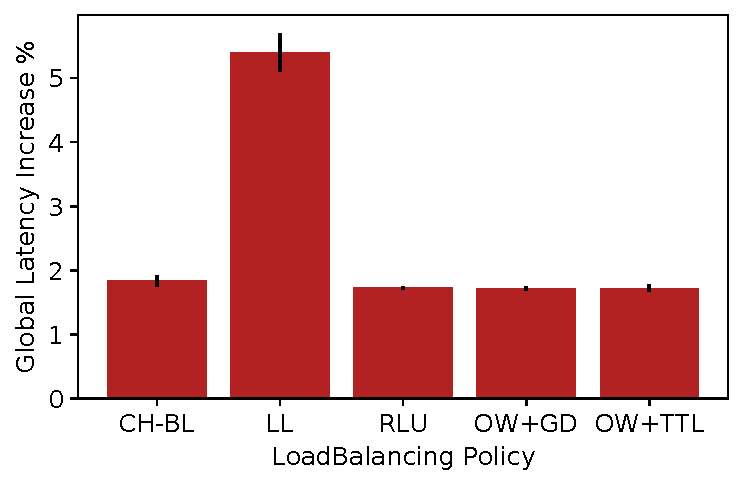
\includegraphics[width=0.5\textwidth]{chrlu/faaslb-osdi22/figs/compare/20-global-latencies-cntnorm.pdf} \label{fig:20-normalized-latencies}}
  \subfloat[Invocation Throughput]{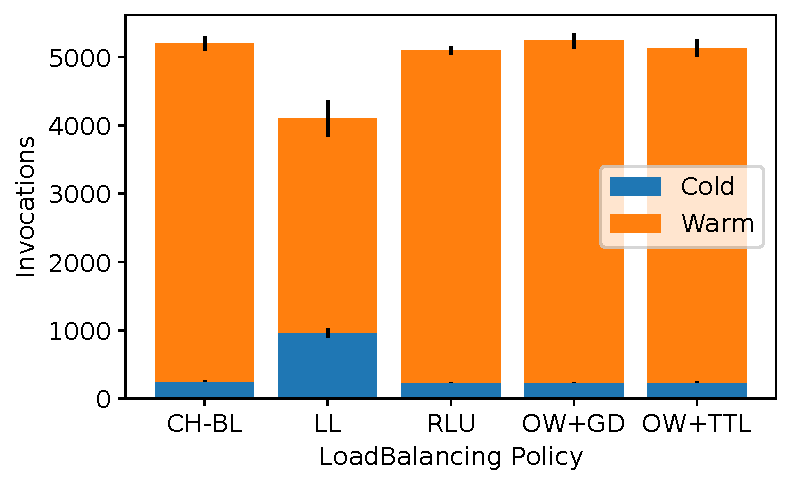
\includegraphics[width=0.5\textwidth]{chrlu/faaslb-osdi22/figs/compare/20-invokes-ttl.pdf} \label{fig:20-invokes}}
 % \vspace*{-0.5cm}
  \caption{Latency and throughput under low-load. Locality-agnostic least-loaded policy has more cold starts and a higher impact on latency.}
  \label{fig:low-load}
\end{figure}


\noindent \textbf{HW and SW Config.}
We run OpenWhisk in a distributed mode across 9 VMs.
8 invokers are each in their own VM with 16 vCPUs and assigned to use 32 GB RAM for hosting functions.
The final VM hosts the controller, load-balancer, and remaining services, with 12 vCPUs and 50 GB RAM to ensure it is not a bottleneck.
Metrics about system load were captured every 5 seconds by calling \textit{uptime} on each invokers VM and normalized by the number of CPUs on that system.
All latency information was recorded by the client, timing the HTTP request until the request completed. 
%
We make no policy changes to the invoker eviction policy, but use the changes from FaasCache~\cite{faascache-asplos21} for eviction decisions on the invoker.

\noindent \textbf{Contenders.}
In addition to our proposed load balancing policy, we compare against the default OpenWhisk load balancing policy (described in Section~\ref{subsec:ch}) with GreedyDual (OW+GD) and 10 minute Time-To-Live (OW+TTL) eviction policies, and implement two other load balancing polices for comparison: least loaded (LL), and consistent hashing with bounded loads using stale load-averages (CH-BL). 
For CH-RLU and CH-BL, we set the $max\_chain\_len=3$, a high max load bound, $b\_max= 6$, and a popularity threshold, $p=20\%$. 
We did not find performance to be particularly sensitive to the load-bound: the function latencies showed little changes across load upper-bounds of $[2-8]$. 
% This is also shown earlier in our latency vs. load analysis in Section~\ref{subsec:function-perf}. 

% $bounded\_ceil = 6$ because of the low correlation between a function's latency and server load from 


%%%%%%%%%%%%%%%%%%%%%%%%%%%%%%%%%%%%%%%%%%%%%%%%%%

\noindent \textbf{Metrics.}
%Evaluating the quality of a serverless load balancing policy can be done using several metrics.
We examine three main metrics: cold starts, the global average latency across all invocations, and the evenness with which load is spread amongst workers.
%
The first two directly and obviously relate to end user service quality but the third is more intricate. 
Providers pay for servers to run functions on and don't want those resources going unused and therefore wasted.
Equally, a server that is overloaded (not enough CPU or memory resources) will cause a spike in end user latency due to contention of queuing.
%
To quantify the global impact on latency from placement decisions, we normalize each invocation's latency by the ideal (minimum) latency, take the per-function mean of these, multiply each mean by the percentage of invocations that function had in the whole trace, and finally take the mean of those function latency means.
This is essentially a weighted average of latency-increase (i.e., slowdown).
It gives some balance between outcomes, for example, a rare function may get several bad placement decisions and thus increase the global latency, or a very common function generally has warm hits and does not impact latency. 
%With this metric we get a specific percentage of the increase in latency that load balancing policies have over the theoretical optimal in which all invocations have their minimum runtime.

% Setup:
% Custom OpenWhisk run on self-hosted VMs
% 8 invokers with 16 vCPUs and assignedto use 32 GB RAM for hosting functions
% Other services on 9th VM with 12 vCPUs and 50 GB RAM.


\begin{figure*}%[ht] 
  \centering
  \subfloat[Latency]{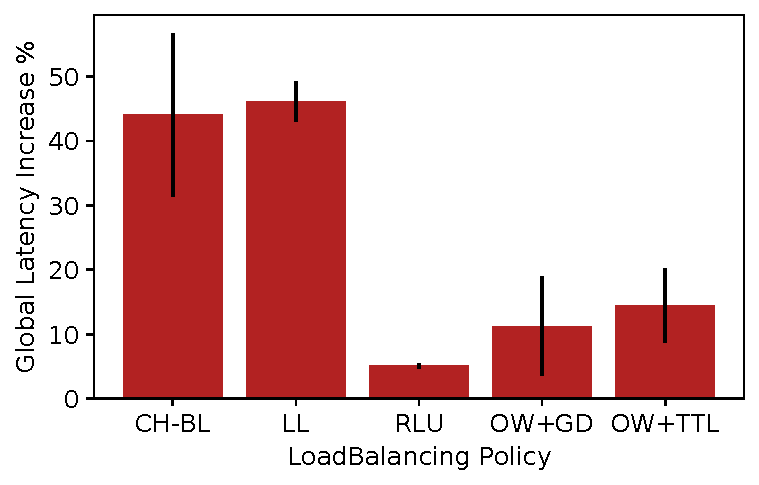
\includegraphics[width=0.4\textwidth]{chrlu/faaslb-osdi22/figs/compare/120-global-latencies-cntnorm.pdf} \label{fig:120-normalized-latencies}} 
  \hfill
  \subfloat[Throughput]{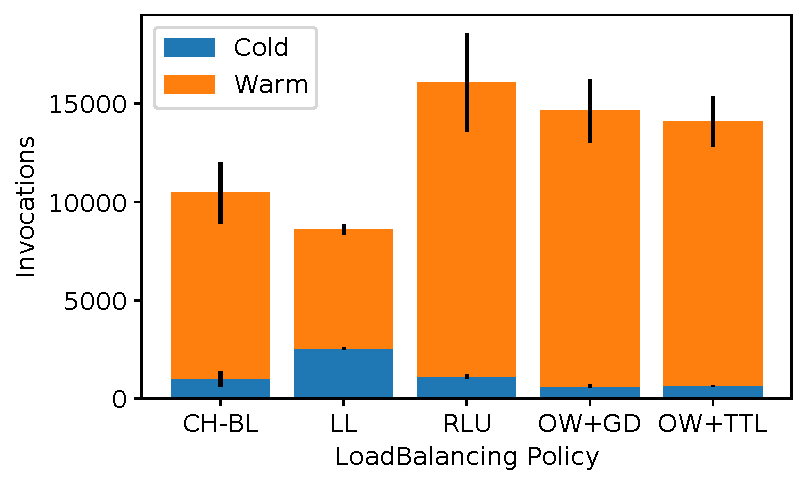
\includegraphics[width=0.4\textwidth]{chrlu/faaslb-osdi22/figs/compare/120-invokes-ttl.pdf} \label{fig:120-invokes}}
  \hfill
  \subfloat[Server Load variance]
  {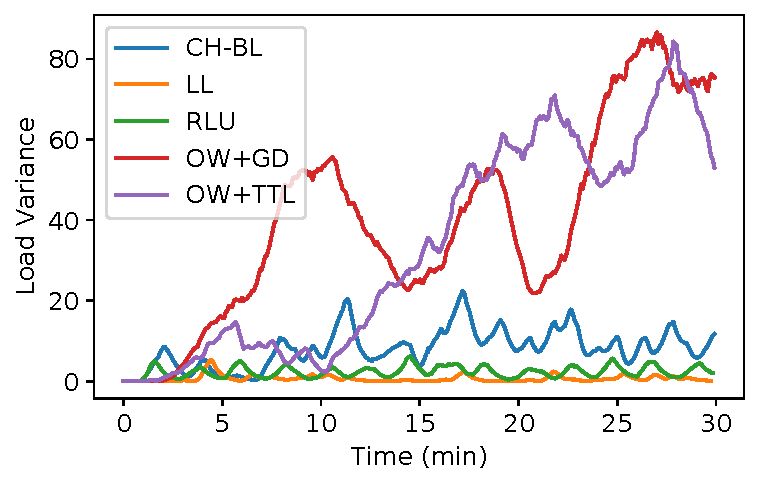
\includegraphics[width=0.4\textwidth]{chrlu/faaslb-osdi22/figs/compare/3-120-loadAvg-variance.pdf} \label{fig:120-load-variance}}
 % \vspace*{-0.5cm}
  \caption{At high server loads, our RLU policy reduces average latency by 2.2x at higher throughput, compared to OpenWhisk's default policy. It does so by keeping cold starts and load-variances low.}
  \label{fig:high-load}
\end{figure*}


\noindent \textbf{Workload.}
We convert 12 functions from FunctionBench~\cite{kim_functionbench_2019} to run on OpenWhisk.
To create a more realistic variety of functions, we create ten copies of each function with unique names, giving us 120 unique functions. 
Each function clone is invoked at different frequencies mimicking the arrival frequencies of the Azure trace~\cite{shahrad_serverless_2020}. 
% We picked these to mimic the invocation disparity shown in real-world traces.
Our load is generated using the closed-loop load generation tool Locust~\cite{locust} to invoke functions, running 20 threads for low load, and 120 for heavy load stressing.
Locust cannot easily have dedicated threads to invoke each function, so we convert the ``frequencies'' into weights and use those to randomly choose what function will be invoked next.
Each thread will iteratively invoke a random function, and after its completion wait 0-1 seconds before invoking another function.
Unless stated otherwise all experiments are run with the above settings, under heavy load, for 30 minutes, and results are the average of 4 runs.

% Workload:
% Load generated by locust
% 50 threads running in closed loop load generation (unless stated)
% 12 functions converted from FunctionBench
% mix of function types, both in runtime and resource usage
% each uploaded 4 times with unique names
% These 4 different ones will be called with diff frequencies of 1, 5, 16, 40
% mimic the invocation disparity displayed in Azure Function trace
% giving us 48 functions to call
% Load applied for 30 minutes. System stable by then and enough for a TTL impact
% each experiment run 4 times, and graphs are the average of those runs, unless stated

\begin{comment}
\subsection{Function Jitter}

\label{sec:unstable-latency}
This system added latency instability combined with the initial cold start overhead for a function's first run are two overheads no load balancing policy can mitigate.
% maybe TODO: Something on on we can only optimize warm hits and server load impact on runtime and will always have "added latency" over the optimal.

To see how our functions' latencies are affected by the system under load, we adjust the setup to have a single invoker and slowly crank up the number of threads making requests to increase the load on that invoker.
Latency increases due to load come from two causes: 1) CPU contention increases function execution time and 2) the server marshalling resources to run the function and extract results.
Figure~\ref{fig:LatencyVsLoad} shows a representative selection of functions, and the latency of individual invocations in relation to the load of our single invoker when they were invoked.
One mixed CPU and disk bound load performing web serving in Figure~\ref{fig:CHAM} sees \textit{no} impact at extreme loads.
Its only latency outliers are due to the inconsistent system overhead we saw above.
A more CPU intense function performing AES key encryption and decryption in Figure~\ref{fig:AES} roughly has some correlation with load.
Once the load gets above \textbf{8} does it not finish near its minimum latency anymore.
The AES function also exhibits layency inconsistency from the system like 'float' did, with many of the invocations under the extreme load of 10 taking as long as invocations with no load.
% Both~\ref{fig:AES} and~\ref{fig:FLOAT}, both CPU bound functions, see \textit{no} impact at extreme loads.
Finally, the long running and CPU bound Sklearn training function in Figure~\ref{fig:TRAIN} is marginally affected as load becomes extreme.
There is a definite correlation between the two, but it is clearly not linear, with a normalized load of 10 only causing a 1.5x increase in function latency.
These results challenge the traditional notion that functions are strictly limited by CPU resources. %, but we see that this isn't true.
We can favor locality more than load, allowing us to both prevent cold starts and not increase latency on warm starts.
Knowing that functions can withstand high server load up to a point, for all our following experiments we set the load bound used by RLU to 6.

\end{comment}


  %\vspace*{-0.2cm}
\subsection{Load-balancing Performance}
\label{sec:policy-comare}

% Policies being compared:
% Ours
% Bounded Loads
% Least loaded
% OpenWhisk (memory sharding) + GD
% OpenWhisk (memory sharding) + TTL

% Lots of metrics to consider when deciding a 'good' policy
% Classic cold start %
% function throughput 
% aggregated function latency
% distribution of load
%   resource usage on invokers

% The quality of a load balancing can be demonstrated in many different ways, and the addition of serverless workloads makes it more complicated.
% Our fixed-time and closed-loop load allows us to examine key metrics for FaaS and load balancing policies in general.


% global normalized latencies for 120 as a percentage over ideal
% ['CH-BL', 'LL', 'RLU', 'OW+GD', 'OW+TTL']
% [44.03687355782084, 46.12511623486831, 5.08886752197281, 11.27379780859461, 14.4173988318167]

% global normalized latencies for 20 as a percentage over ideal
% ['CH-BL', 'LL', 'RLU', 'OW+GD', 'OW+TTL']
% [1.83828219306087, 5.397093279722829, 1.7271133329324055, 1.7177648275920407, 1.723332172907966]

% Stable load
% Compare functions w/20 threads
% 20-compare-functions-ShardingContainerPoolBalancer-RLULFSharding.pdf 0.9997180360888229
% 20-compare-functions-LeastLoadBalancer-RLULFSharding.pdf 2.6262500335629335
% Compare functions w/120 threads
% 120-compare-functions-ShardingContainerPoolBalancer-RLULFSharding.pdf 1.7029922705698093
% 120-compare-functions-LeastLoadBalancer-RLULFSharding.pdf 7.805708861373892

When we run them under \textbf{light load} in Figure~\ref{fig:low-load}, the policies that use a locality mechanism are essentially identical.
The load on any one server is never high enough to impact co-located functions and we never have to forward invocations and incur excess cold starts, giving us a \quotes{lower bound} on load balancing.
The low 1-2\% latencies in Figure~\ref{fig:20-normalized-latencies} we see here are due to initial cold starts for functions and the varied overhead imparted by the system analyzed earlier.
The least loaded policy is significantly worse as it's lack of locality causes excessive cold starts as evidenced by the high number of cold starts in its invocation results detailed in Figure~\ref{fig:20-invokes}.
% The global latency impact in Figure~\ref{fig:20-normalized-latencies} and invocation throughputs in Figure~\ref{fig:20-invokes} 


Next we run the policies under our \textbf{heavy load} scenario, and get a clear distinction between how each of them performs. 
The two versions of OpenWhisk  in Figure~\ref{fig:120-normalized-latencies} only increase latency by 11\% and 14\% respectively which is rather good.
They cannot complete with RLU whos increase is less than half of that, a tiny 5\% impact on global latency.
CH-BL and least loaded increase global latency by over 40\%, showing terrible performance in that metric and on invocation throughput. 


The wide gap between policies can be understood by comparing the load variance between their workers (Figure~\ref{fig:120-load-variance}).
OpenWhisk's default policy is to only move a function to another server if the ``home'' one does not have available memory to run it. 
While very good for locality (getting fewer cold starts than RLU in Fig~\ref{fig:120-invokes}), it creates severe imbalance on the worker loads.
A few workers grow to extremely high load and their functions suffer, while others are mostly empty. 
RLU intelligently forwards invocations when a worker is near overload, keeping load variance low while protecting locality. 
Least loaded actually does the best at keeping equal load amongst workers, but at the cost of poor locality.

% An important seconday goal is to full utilize worker resources and ensure that certain workers are neither over- nor under-loaded compared to each other.
% The default OpenWhisk policy does a poor job of keeping load even on its workers, as shown in Figure~\ref{fig:OW-loadavg}
% Several workers have a load near 0, and one has a load of over 10!
% While the system has a stable mean load denoted by the solid black line, the dashed variance line is always extremely high.
% Our policy, shown in Figure~\ref{fig:Forward-loadavg} has a similar mean load to that of OpenWhisk, hovering just under 2.
% It differs by having a substantially lower variance, keeping invoker CPU load close together.
% For example invoker 4, the purple line, reaches a load of 4x at points but the system forwards work to other invokers and the load stabilizes.

%  \vspace*{-0.2cm}
\subsubsection{Handling Bursty Traffic}

% Two of the high-frequency functions have their frequency quadrupled and returned to normal every 10 seconds
% aes and gzip specifically, CPU and disk/cpu intensive respectively


\begin{figure}
  \centering
  \subfloat[Global Latency Impact]{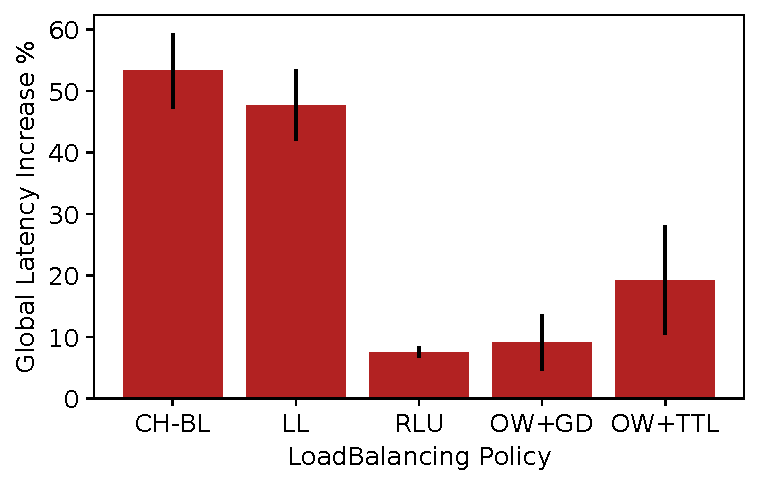
\includegraphics[width=0.5\textwidth]{chrlu/faaslb-osdi22/figs/bursty/120-global-latencies-cntnorm.pdf} \label{fig:bursty-latencies} }
  \subfloat[Worker Load Variance]{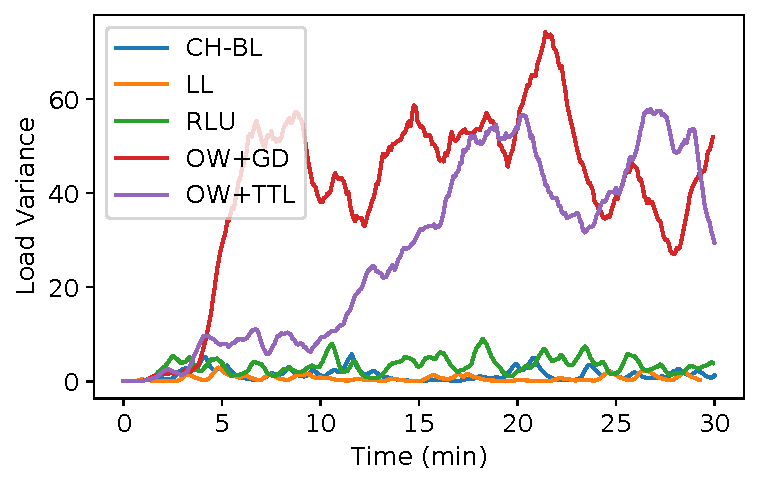
\includegraphics[width=0.5\textwidth]{chrlu/faaslb-osdi22/figs/bursty/3-120-loadAvg-variance.pdf} \label{fig:bursty-variance} }
%  \vspace*{-0.4cm}
  \caption{RLU improves latency by 10\% compared to OpenWhisk under bursty load conditions, while keeping a low worker load variance.}
  \label{fig:bursty-closedload}
\end{figure}


% Bursty load, 120 threads
% 120-compare-functions-ShardingContainerPoolBalancer-RLULFSharding.pdf 1.0932351152955206
% 120-compare-functions-LeastLoadBalancer-RLULFSharding.pdf 6.784717290259041

% global normalized latencies for 120 as a percentage over ideal
% ['CH-BL', 'LL', 'RLU', 'OW+GD', 'OW+TTL']
% [53.31502690829111, 47.720802127692316, 7.542333155555457, 9.089841768309597, 19.267038417080776]

\begin{figure}
  \centering
  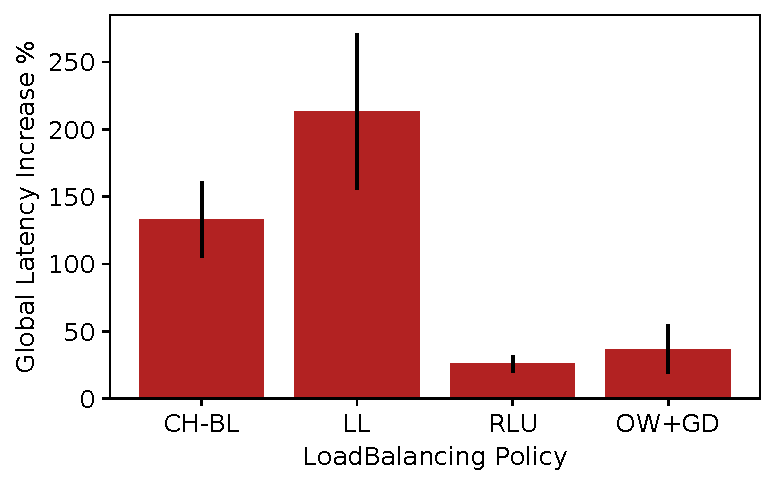
\includegraphics[width=0.6\textwidth]{chrlu/faaslb-osdi22/figs/ow/openload/openload-latencies-cntnorm.pdf}
 % \vspace*{-0.3cm}
  \caption{Global latency impact under a 30-minute long rising burst load from an open-loop generator. RLU reduces  latency by 17\% compared to OpenWhisk.}
  \label{fig:bursty-openload}
 %   \vspace*{-0.3cm}
\end{figure}

Next we take two different bursty workloads to see how the polices handle changes in invocation patterns.
The first uses the same closed-loop load generation but adjust the weights by which functions are invoked.
Every 30 seconds two of the top weighted functions are chosen to become bursty, and have their weights set much higher.
At the end of a burst their weights are returned to normal and another two functions are chosen.
As can be seen in Figure~\ref{fig:bursty-latencies} our policy acheives a 17\% lower impact on global latency than OpenWhisk with GreedyDual.
RLU represents a 60\% reduction to latency over OpenWhisk with its default TTL backend.
The more advanced eviction decision choices have a clear effect on improving the system even when the load balancer does not optimize for it.
The longer running functions in our workload have a larger effect on system load and the load balancer must be aware of this impact and either spread that heavy popular function around or move other functions off of that server.
Again, OpenWhisk does not take load into account and severely overloads some servers while languishing others.
We see more sky-high load variances from this bursty workload in Figure~\ref{fig:bursty-variance}.
Policies that monitor load, our RLU, CH-BL, and least loaded keep tighter control on load variance.

% We do suffer more cold starts, caused by moving traffic across workers to avoid load spikes from the bursty workloads.
% OpenWhisk does not try to mitigate variable workloadsd and suffers accordingly. 

% global normalized latencies for open load generation
% ['CH-BL', 'LL', 'RLU', 'OW+GD']
% [140.53344802991816, 228.83239333263217, 25.886003912929013, 36.857319393171736]

The second busrty load is a 30 minute long-rising burst, starting with just a few invocations per second and reaching a sustained peak of roughly 18 invocations per second at roughly 25 minutes.
We generated this load with a custom open-loop load tool that fires invocations but does not block waiting for completion.
New invocations are continually fired in a preset pattern of function types and times.
The global latency impact of this final scenario can be seen in Figure~\ref{fig:bursty-openload}.
Only the final 10 minutes of the workload place the system under extreme load, and the differences between policies reflect this.
CH-BL and least loaded cannot keep up with the suddenly changing load, causing a latency increase of over 100\% and 200\% respectively.
RLU's 25\% increase in global latency is still significantly better, 30\% lower, than OpenWhisk.
Our policy is able to make ideal choices for function placement under a varient of realistic workload scenarios.

\subsubsection{Scaling}
\begin{comment}
\begin{figure}
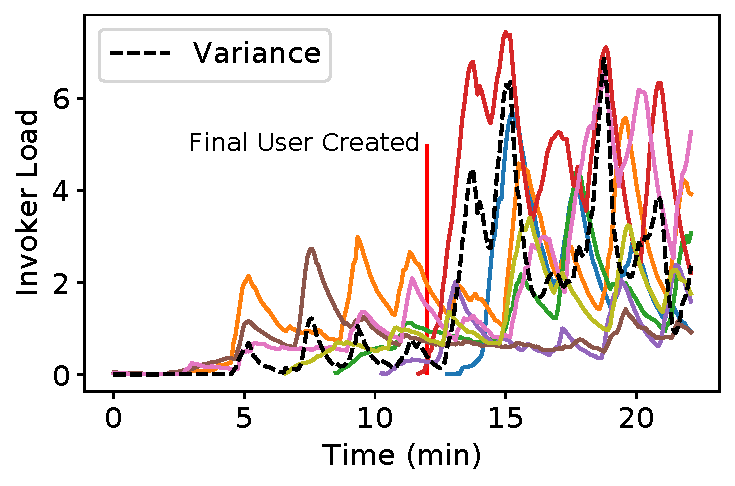
\includegraphics[width=0.33\textwidth]{../figs/scaling/120-loadAvg-6sec.pdf}
  % \vspace*{-0.3cm}
  \caption{When load increases over time, new workers are spun up and recieve a share of the workload while not being overloaded.}
  \label{fig:scaling}
%\vspace*{-0.3cm}
\end{figure}
\end{comment}

\begin{figure}  
  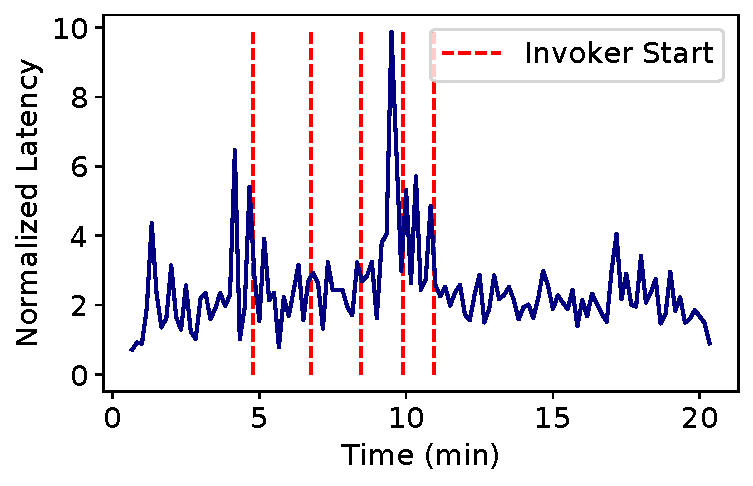
\includegraphics[width=0.6\textwidth]{chrlu/faaslb-osdi22/figs/scaling/scaling_lat_over_time-nolabel.pdf}
%  \vspace*{-0.3cm}
  \centering
  \caption{The average normalized function latency over time for a dynamic workload. New invokers are launched at the dashed lines, keeping the latency in check.}
  \label{fig:scaling-latency}
%  \vspace*{-0.3cm}
\end{figure}


% we are able to scale up infrequently and well
% system handles load as if all invokers were always up

% As described in Section~\ref{}, we can intelligently scale our systems workers as demand increases.
Lastly we want to demonstrate how our policy reacts to scaling the number of workers as demand increases.
We start our cluster with only 3 invokers and increase applied load up to the heavy load scenario above.
Rather than starting with the 120 threads of the heavy load with this smaller cluster, we adjust the scenario to start with a single thread and add a new one every 6 seconds, reaching the final thread count at about minute 12.
% Our small cluster does not allow us to match the multi-server scaling up and down changes of the simulator, so here we turn on invokers when there is an increase in forwarding to server servers beyond the 'home' server.
%The results for a single run of this scaling are in Figure~\ref{fig:scaling} with each invoker being represented by a unique color.

As the average invoker load increases, the controller activates a new worker and starts directing work towards it.
New workers are kept under the load bound of 6 and see load similar to our previous experiments that had a constant load.
%We can also correlate when new invokers are started to the latency invoked functions are encountering.
Figure~\ref{fig:scaling-latency} shows the function latencies (normalized to respective min. warm times). % and average them in 5 second groups. 
Preceeding each worker being started is a rise in overall latency, which then falls after the invoker has come online and starts taking additional load.
Thus, our horizontal scaling is able to dynamically keep the function latency in check, even though it only uses coarse-grained server load metrics.

% The remaining 5 workers are started dynamically, and quickly have a load similar to already existing workers.
% There are not load spikes or troughs, indicating the work is being spread well to new invokers as time moves on.
%These graphs are not a combination of multiple runs, but are characteristic of the performance across runs.

%\vspace*{-0.2cm}
\subsubsection{Load-balancer Overhead}

% BoundedLoadsLoadBalancer: 0.0001106853074066166
% LeastLoadBalancer: 6.170695498725195e-05
% RLULFSharding: 0.0001242685814681948
% ShardingContainerPoolBalancer: 4.7238211672012455e-05

More complicated routing decisions naturally mean they are more computationally expensive to perform.
% We have been able to keep balancing decisions to roughly 1 ms thanks to the optimizations described in Section~\ref{sec:impl}. 
Even so, RLU is on significantly slower making individual routing decisions, taking on average $1242.6 \mu$s to OpenWhisks' $472.3 \mu$s.
Such times represent a fraction of the time spent per-request by the system and is made up for by our more optimal placements. 


% %\vspace*{-0.3cm}
\subsection{Simulation Evaluation}
\label{subsec:eval-sim}


  \begin{figure}
  \centering
  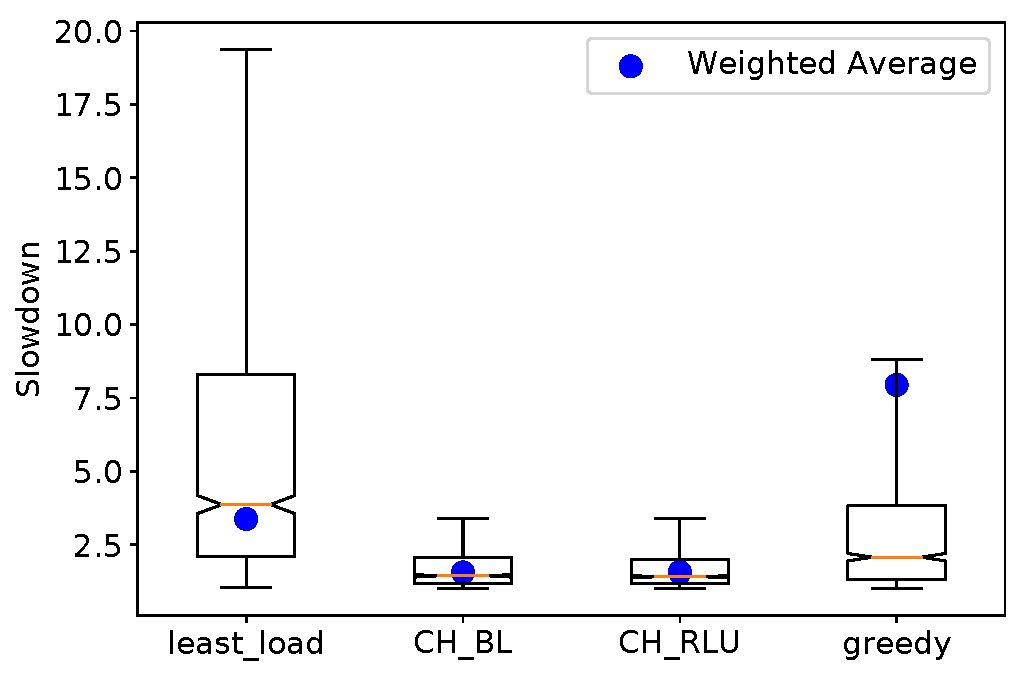
\includegraphics[width=0.3\textwidth]{chrlu/faaslb-osdi22/figs/1k/latencies-GD.pdf}
%  \vspace*{-0.3cm}
  \caption{[Simulated] Function latency distribution. }
  \label{fig:1k-lat}
%  \vspace*{-0.3cm}
  \end{figure}

\begin{figure}
  \centering
  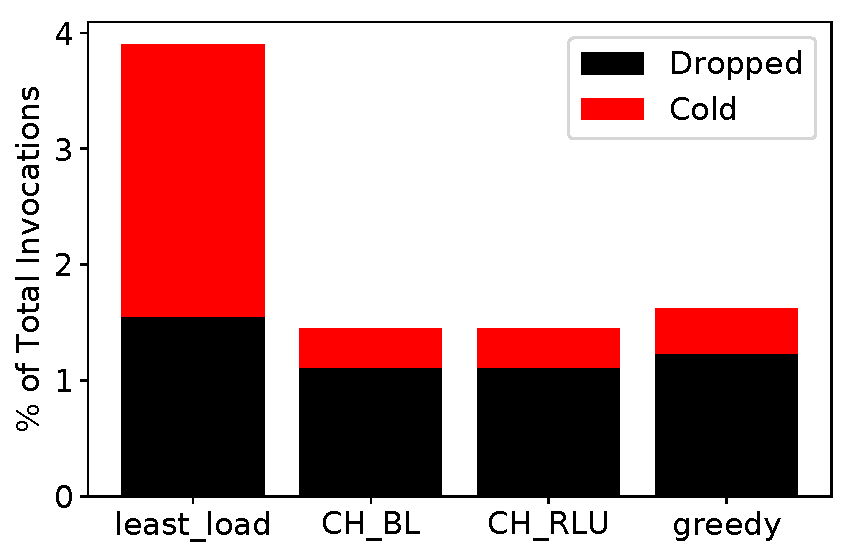
\includegraphics[width=0.3\textwidth]{chrlu/faaslb-osdi22/figs/1k/cd-GD.pdf}
%    \vspace*{-0.3cm}
  \caption{[Simulated] Cold and dropped functions.}
  \label{fig:1k-cd}
%    \vspace*{-0.3cm}
\end{figure}


To investigate the performance of various load-balancing policies at larger scales, we use a simulation approach.
We have developed a discrete-event simulator, which plays a function workload trace, and emulates the various aspects of function execution and slowdown: slow/warm starts, slowdown due to concurrent processing by emulating a G/G/k queuing system on each server, and various load metrics (emulating Linux exponentially decaying load averages, stale loads, real-time loads, etc.). 
The simulator allows us to implement different policies using information that would not otherwise be available on a real system: accurate function cold and warm times, instant load information, etc.
The function running times are computed by adding the actual provider-captured running times to the OpenWhisk and Docker startup overheads that are empirically measured and modeled.
This, when combined with queuing delays, captures the overall slowdown due to concurrent processing.
The simulator is implemented in Python in about 3,000 lines of code. 

We run the Azure trace with 1000 randomly chosen functions spanning almost a million invocations, and compare different load-balancing policies.
This workload is highly bursty and is characterized by the Figures in Section~\ref{sec:challenges}. 
We have implemented a ``online greedy optimal'' policy that considers \emph{all} servers when running functions, by picking the server with the lowest expected running time (based on Section~\ref{subsec:chch}).
This would be impractical and unrealistic to implement, since it needs accurate information about every function's keep-alive status on every server, and an accurate model of function performance at various loads.
Nevertheless, it provides an optimistic baseline: our consistent-hashing based policy ($CH-RLU$) is significantly simpler, only considers a small subset of servers, and does not require omniscient cluster state. 

Figure~\ref{fig:1k-lat} compares this greedy policy with a locality-agnostic ``least-loaded'' policy that is popular in web-clusters, and the two consistent-hashing based policies. 
The figure shows the function slowdown factor for each function, as well as the global average slowdown.
Slowdown is defined as the ratio of function's execution time to its base warm time without any system overhead, resource contention, or queuing delays.
Most functions do poorly with the least-loaded policy: the median function slowdown is almost $4\times$, primarily because of high cold-starts.
Figure~\ref{fig:1k-cd} compares the cold and dropped statistics for the various policies.

Returning to Figure~\ref{fig:1k-lat}, both CH-BL and CH-RLU have comparable performance, with a median slowdown of $2.4$. 
Finally, and surprisingly, the omniscient greedy policy performs poorly: with the global slowdown approaching $7$.
The primary reason for this is because of the bursty nature of the workload: the greedy policy tends to pick the server with the least-loaded server that can run the warm function.
However because of stale load information, we see a \emph{herd effect} on the server, and this causes extremely high resource contention and latency, even though the number of cold-starts is small (compared in Figure~\ref{fig:1k-cd}). 


% \begin{centering}
\begin{figure}
  \centering
  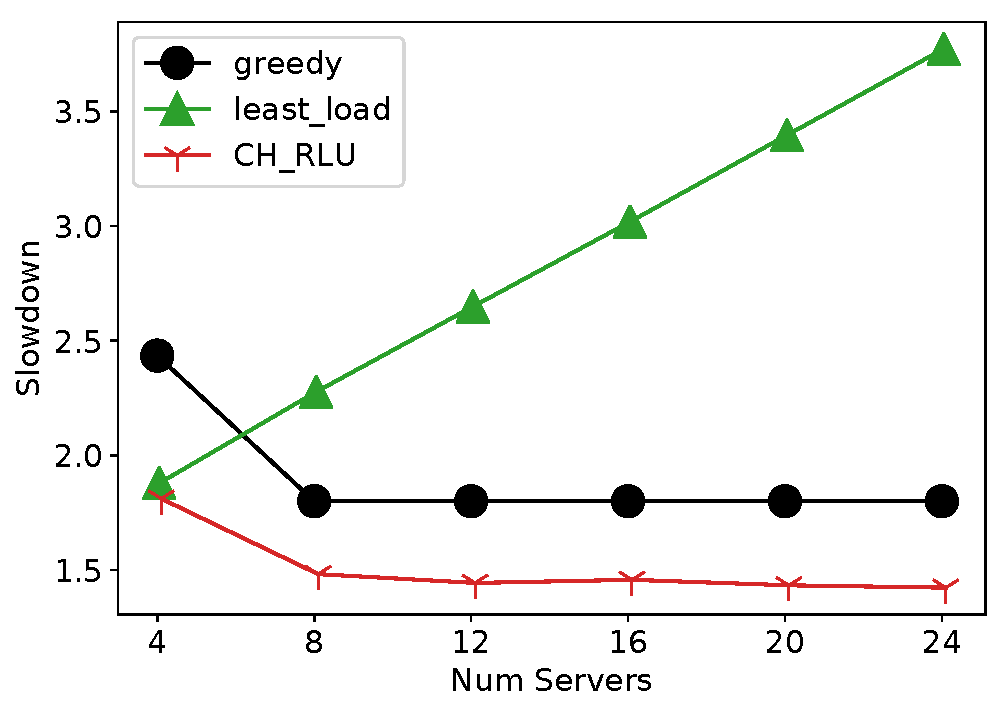
\includegraphics[width=0.3\textwidth]{chrlu/faaslb-osdi22/figs/1k/latencies-250scaling.pdf}
  %  \vspace*{-0.3cm}
  \caption{[Simulated] Function latencies as cluster size is increased. Least-loaded performs \emph{worse} because its locality and cold-starts become worse as more servers are added.}
  \label{fig:1k-scaling}
 %   \vspace*{-0.3cm}
\end{figure}
% \end{centering}

Finally, we investigate performance when the cluster size changes.
Figure~\ref{fig:1k-scaling} shows the slowdown for the three policies when the number of servers is increased.
Importantly, the total number of computing and memory in the cluster is kept constant at 256 CPUs and 512 GB, and the size of the individual servers is changed.
Thus 4 servers with 64 CPUs are compared with 8 servers with 32 CPUs, etc.
This experiment is intended to capture the effects of locality: smaller number of servers may have a higher hit-rate, and a more even load-spread.

Figure~\ref{fig:1k-scaling} shows how the function slowdown for both CH-RLU and greedy decays as the number of servers is increased.  
This is because larger servers see heavier lock and other resource contention, and thus while they may exhibit better locality, the load-induced slowdown dominates.
This has important ramifications for large FaaS providers, since they can continue using smaller servers for running functions, and expands the utility of small deflatable/harvestable VMs for running colocated functions~\cite{serverless-harvest-sosp21}.

CH-RLU reduces the function slowdown by 20\% compared to the greedy approach, across a wide range of cluster configurations in Figure~\ref{fig:1k-scaling}. 
Interestingly, least-loaded's performance worsens with increasing number of servers and fragmentation.
The main culprit is worsening locality.
With a small number of servers, least-loaded can get ``lucky'' and score a keep-alive cache-hit.
These fortuitous warm-starts get less probable with an increasing number of servers. 

%%% Local Variables:
%%% mode: latex
%%% TeX-master: "paper"
%%% End:




\section{Related Work}

\subsection{Load Balancing Related Work}

\begin{comment}
\noindent \textbf{FaaS Resource Management.}
The initialization overheads of serverless functions and their repeated invocations have spawned a great deal of research into optimizing their resource management.
Recent surveys~\cite{faas-survey-jan-2022, raza2021sok, eismann2020serverless, hassan2021survey, mampage2021holistic} provide an overview of the challenges and solutions in this very active research area. 

Reducing the overhead of serverless functions through various systems and virtualization-level mechanisms and  optimizations~\cite{du2020catalyzer, firecracker-nsdi20, dukic2020photons, akkus_sand_2018, vhive-asplos21, carreira2021warm}. 
%
Locality for FaaS resource management has been explored in the form of function keep-alive policies~\cite{shahrad_serverless_2020}. 
Our work builds on and uses the caching-based Greedy-Dual policy from FaasCache~\cite{faascache-asplos21}. 
%
Single-server environments have been the focus of these mechanisms and policies: we have made an initial attempt to understand their interactions in a distributed cluster context.
%
Inter-function dependencies can also be used for predictive resource management and reducing function communication and startup costs~\cite{gunasekaran2020fifer, daw2021speedo, shen2021defuse}: incorporating these policies into our load-balancer is part of future work. 
\end{comment}

% \noindent \textbf{Function Load Balancing:}
Package-aware load balancing~\cite{package-cristina-19}  identifies and uses function code dependencies (software packages) as an important source of data locality.
While this is an important factor, we focus on in-memory locality of kept-alive functions, since memory capacity is much smaller than permanent storage and caching functions in memory has a very large performance impact.
%
CPU contention and interference is a major source of performance bottlenecks for co-located functions, and adjusting CPU-shares using cgroups can provide significant benefits~\cite{suresh2019fnsched, suresh2021servermore, ensure-faas-acsos20}.
%
The load-locality tradeoff we explore is complementary to these CPU scheduling optimizations. 
%
The repetitive nature of functions and their workflows can also be used to improve resource utilization and latency~\cite{hunhoff2020proactive, yu2021faasrank, puru_xanadu_20, przybylski2021data}: our load-balancer is stateless for the sake of simplicity and can be enhanced with these techniques if necessary.


The tradeoff between locality and performance has also been explored in the context of delay scheduling~\cite{zaharia2010delay} for data-parallel applications like MapReduce.
Load-balancing is seen as a ``dispatch'' problem in queuing theory, and the FaaS cluster system most closely approximates G/G/PS, since the arrivals and service times are not markovian.
Techniques such as ``join the shortest queue'', and ``least work left''~\cite{gupta2007analysis} have been shown to be effective.
The online-greedy policy evaluated in the previous section closely approximates least-work-left.
However, it is difficult to implement in practice since the running times of functions is hard to predict due to their volatile arrival distribution mixtures and high variances in running time due to various system interference effects.



% In general, 
% CH, dynamo,
% CH-RJ not applicable because of lack of locality.
% Stale loads dahlin, mitzen,
% power of 2 choices: but not locality aware and load has an uncertain bearing on performance.
% \subsection{Queuing and Dispatch}
% Remaining time times the original size (RS) ~\cite{scully2022bounding}
% Guardrails:~\cite{}
% Although we focus on the heavy-traffic regime with server loads far exceeding one. 

%%% Local Variables:
%%% mode: latex
%%% TeX-master: "paper"
%%% End:


\subsection{QoS Related Work}

% \noindent\textbf{FaaS Resource Management:}
% Multiple recent projects have looked into ways for optimizing the resource management of serverless frameworks, including solutions that
% reduce the overhead of the cloud functions~\cite{du2020catalyzer, firecracker-nsdi20, dukic2020photons, akkus_sand_2018, vhive-asplos21, carreira2021warm},
% improve locality through keep-alive policies~\cite{Shahrad:ATC:2020:ServerlessInTheWild},
% better caching algorithms for worker nodes~\cite{faascache-asplos21},
% reducing function communication and startup costs~\cite{gunasekaran2020fifer, daw2021speedo, shen2021defuse}, among others. 
% Our work leverages the caching-based Greedy-Dual policy~\cite{faascache-asplos21}, in a cluster with pools that support differentiated services for high- versuls low-priority functions.

% \noindent\textbf{Latency-sensitive scheduling and load balancing in serverless:}
% Nightcore~\cite{jia2021nightcore} provides low end-to-end latency and variability using fast paths for internal calls, low-latency message channels, efficient threading and concurrency.
% Atoll~\cite{singhvi2021atoll} uses deadline-aware two-level scheduling as part of a low-latency serverless platform.
% Our proposal can be added to those solutions to further implement differentiated services on top of more performant serverless platforms.
% In general, there is a rich previous body of work in performance improvement methods~\cite{soakes_sock_2018,kaffes2019centralized,hunhoff2020proactive} that are complementary to our approach.
% In addition, we extend the notion of locality-aware function routing~\cite{firecracker-nsdi20,aumala2019beyond,abdi2023palette} and use it within cluster pools that ensure differentiated services when functions can be divided into priority classes. 

\mhead{Differentiated services in serverless}
Sequoia~\cite{Tariq:SOCC:2020:Sequoia} is a serverless framework with a QoS scheduler based on a simple priority-based queue; however, the issue of starvation in the presence of a continuous arrival of high-priority functions is not considered.
Furthermore, the framework is based on a completely new design that does not support synchronous function calls.
In contrast, our solution was implemented on top of OpenWhisk and considers both synchronous and asynchronous functions.
Bilal et al.~\cite{Bilal:CoRR:2021:GreatFreedom} analyzed the trade-off space between performance and cost that arises from different CPU/RAM configurations and the resulting function performance.
This approach is orthogonal to ours and can be leveraged by the provider to offer differentiated services that span this configuration space.
Qiu et al.~\cite{Qiu:WOSC:2021:LatencyCritical} suggested that providers could implement resource over-commitment for FaaS workloads with loose latency objectives;
our approach ties over-commitment with current demand, with a dynamic mechanism that supports handling of bursts in high priority workloads at the expense of low priority ones.
\emph{Real-time serverless}~\cite{Nguyen:WoSC:2019:Real-Time} is a work-in-progress system that describes an interface for specifying invocation rate guarantees and proposes delivering them via admission control and predictive container management.

% \noindent\textbf{Workload shifting in the cloud:}
% Delaying of tasks has been proposed to make better use of renewable excess energy~\cite{Wiesner:Middleware:2021:TemporalShifting,Wiesner:EuroPar:2022:Cucumber}, to reduce
% energy consumption for workflow execution~\cite{Versluis:HotCloudPerf:2022:TaskFlow}, among others.
% While we have not implemented policies with energy management goals, our solution could be extended to consider energy information (peaks, variable costs, green energy availability).

\mhead{Multi-pool cluster scheduling}
Virtual cluster pools have been used for dynamic resource management in datacenters~\cite{Chase:HPDC:2003:COD}, to handle increased workloads in data analytics clusters~\cite{Lee:HotCloud:2011:Heterogeneity-Aware}, for QoS multi-class admission control~\cite{Delimitrou:ICAC:2013:ARQ}, and to decrease the delays of scheduling decisions~\cite{singhvi2021atoll}. 
We use this technique for service differentiation, and complement it with a novel control-based dynamic resizing mechanism to support burst absorption in serverless workloads.
%Note: {Lee:HotCloud:2011:Heterogeneity-Aware} uses too pools: core nodes and accelerator nodes; the latter are temporarily added to the cluster to handle increased jobs (observed or anticipated).

\mhead{Current Status of Differentiated FaaS Invocations}
\label{sec:motivation:currentStatus}
A recent empirical study~\cite{Tariq:SOCC:2020:Sequoia} found that current cloud providers (AWS, Azure, GCP and IBM) treat HTTP functions differently from those triggered by other means, frequently via undocumented behavior, including different concurrency limits and prioritization versus background functions.
In addition, while asynchronous functions are queued and thus the user understands that they may not execute immediately, providers don't typically enqueue synchronous functions but rather return with an error if peak exceeds concurrency limits or provider capacity.\footnote{An exception is GCP which handles synchronous calls in best effort fashion, performing queuing but not ensuring zero drops~\cite{Tariq:SOCC:2020:Sequoia}.}
%
Thus, the major public cloud providers are already implicitly defining two classes of functions: high priority (synchronous) and lower priority (asynchronous), with the latter being delay-tolerant.
%asynchronous functions in AWS can be queued up to 6 hours.\footnote{\url{HTTPs://docs.aws.amazon.com/lambda/latest/dg/invocation-async.html}}
%Asynchronous functions are either explicitly (for example, with the \texttt{async} keyword in OpenWhisk) or implicitly (by its trigger) defined in current platforms.
%The asynchronous functions are good candidates to be delayed if needed.

In OpenWhisk asynchronous functions are defined with the \texttt{async} keyword and follow a different execution path than synchronous ones.
However, the platform does not use any mechanism to delay or execute them at a lower priority.
A solution that treats \texttt{async} functions as delay-tolerant, scheduled with a lower priority than synchronous functions, can be added to OpenWhisk without API modifications.

%
% OLD, conference-paper related work
%
% \noindent \textbf{FaaS Resource Management.}
% The initialization overheads of serverless functions and their repeated invocations have spawned a great deal of research into optimizing their resource management.
% Recent surveys~\cite{faas-survey-jan-2022, raza2021sok, eismann2020serverless, hassan2021survey, mampage2021holistic} provide an overview of the challenges and solutions in this very active research area. 

% Reducing the overhead of serverless functions through various systems and virtualization-level mechanisms and  optimizations~\cite{du2020catalyzer, firecracker-nsdi20, dukic2020photons, akkus_sand_2018, vhive-asplos21, carreira2021warm}. 
% %
% Locality for FaaS resource management has been explored in the form of function keep-alive policies~\cite{shahrad_serverless_2020}. 
% Our work builds on and uses the caching-based Greedy-Dual policy from FaasCache~\cite{faascache-asplos21}. 
% %
% Single-server environments have been the focus of these mechanisms and policies: we have made an initial attempt to understand their interactions in a distributed cluster context.
% %
% Inter-function dependencies can also be used for predictive resource management and reducing function communication and startup costs~\cite{gunasekaran2020fifer, daw2021speedo, shen2021defuse}: incorporating these policies into our load-balancer is part of future work. 

% \noindent \textbf{Function Load Balancing:}
% Package-aware load balancing~\cite{package-cristina-19}  identifies and uses function code dependencies (software packages) as an important source of data locality.
% While this is an important factor, we focus on in-memory locality of kept-alive functions, since memory capacity is much smaller than permanent storage and caching functions in memory has a very large performance impact.
% %
% CPU contention and interference is a major source of performance bottlenecks for co-located functions, and adjusting CPU-shares using cgroups can provide significant benefits~\cite{suresh2019fnsched, suresh2021servermore, ensure-faas-acsos20}.
% %
% The load-locality tradeoff we explore is complementary to these CPU scheduling optimizations. 
% %
% The repetitive nature of functions and their workflows can also be used to improve resource utilization and latency~\cite{hunhoff2020proactive, yu2021faasrank, puru_xanadu_20, przybylski2021data}: our load-balancer is stateless for the sake of simplicity and can be enhanced with these techniques if necessary.


% The tradeoff between locality and performance has also been explored in the context of delay scheduling~\cite{zaharia2010delay} for data-parallel applications like MapReduce.
% Load-balancing is seen as a ``dispatch'' problem in queueing theory, and the FaaS cluster system most closely approximates G/G/PS, since the arrivals and service times are not markovian.
% Techniques such as ``join the shortest queue'', and ``least work left''~\cite{gupta2007analysis} have been shown to be effective.
% The online-greedy policy evaluated in the previous section closely approximates least-work-left.
% However, it is difficult to implement in practice since the running times of functions is hard to predict due to their volatile arrival distribution mixtures and high variances in running time due to various system interference effects.


%%% Local Variables:
%%% mode: latex
%%% TeX-master: "paper"
%%% End:



%~\cite{lbfaas-hpdc2022}

In this chapter we have explored the tradeoff between locality and load for serverless functions. 
Our CH-RLU policy can tackle the challenges of function heterogeneity, workload skew, bursty workloads, and stale loads.
We enhance consistent hashing to yield a simple and practical load-balancing policy. 
Empirical evaluation shows substantial improvements in function latency (by more than $2\times$) compared to OpenWhisk's load balancing strategy.


\begin{comment}
\begin{figure}
  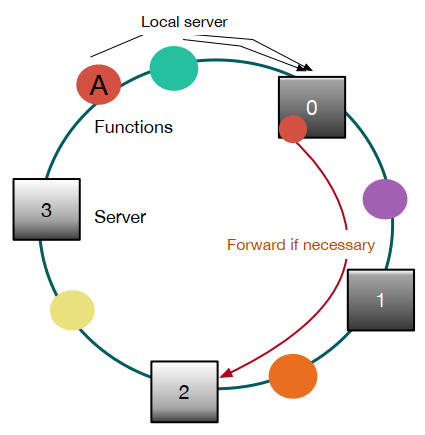
\includegraphics[width=.9\columnwidth]{./figures/consistent-hashing.png}
  \caption{Consistent hashing ring featuring function forwarding~\cite{lbfaas-hpdc2022}.}
  \label{fig:ch-rlu}
\end{figure}

In my work just accepted to HPDC~\cite{lbfaas-hpdc2022}, we take a different approach to load and locality balancing.
% Some functions are more \textit{popular} than others, and therefore will take up more system resources.
Previous work~\cite{shahrad2020serverless} revealed that a few functions make up the lion's share of invocations in FaaS systems.
Per Figure~\ref{fig:serverless-invocations} over 99\% of invocations are from just 19\% of functions, and load balancers need to take this pattern into account.
To start our balancing policy we use consistent hashing to always route a function to a home worker, favoring locality especially for those rarely invoked functions.
In the event a home worker is overloaded, we want to conditionally migrate work to other workers in an affinity-aware manner.
This load based migration locality is achieved by \textit{pushing} work around the has ring as shown in Figure~\ref{fig:ch-rlu}.
As a server's load increases, invocations are randomly pushed around the ring with popular functions being more likely to be forwarded.
This spreads work around preventing load imbalance, maintains locality for functions, and avoids latency increases from high CPU load on any individual worker.
\end{comment}